\documentclass{cmc}

\begin{document}

\pagestyle{fancy}
\lhead{\textit{\textbf{Computational Motor Control, Spring 2019} \\
    Python exercise, Lab 5, GRADED}} \rhead{Students \\ Honigmann, Munier \& Plett Palomar}

\section*{Student names: Honigmann Simon, Munier Louis \& Plett Palomar Kilian Asterio}
\textit{Instructions: Update this file (or recreate a similar one,
  e.g.\ in Word) to prepare your answers to the questions. Feel free
  to add text, equations and figures as needed. Hand-written notes,
  e.g.\ for the development of equations, can also be included e.g.\
  as pictures (from your cell phone or from a scanner).
  \textbf{\corr{This lab is graded.}} and must be submitted before
  the \textbf{\corr{Deadline : 11-04-2018 Midnight}}.  \\ Please
  submit both the source file (*.doc/*.tex) and a pdf of your
  document, as well as all the used and updated Python functions in a
  single zipped file called \corr{lab5\_name1\_name2\_name3.zip} where
  name\# are the team member’s last names.  \corr{Please submit only
    one report per team!}}
\\

\textit{The file \fileref{lab\#.py} is provided to run all exercises
  in Python.
  % Each \fileref{exercise\#.py} can be run to run an exercise
  % individually.
  % The list of exercises and their dependencies are shown in
  % Figure~\ref{fig:files_lab5}.
  When a file is run, message logs will be printed to indicate
  information such as what is currently being run and and what is left
  to be implemented. All warning messages are only present to guide
  you in the implementation, and can be deleted whenever the
  corresponding code has been implemented correctly.}


% \textit{In this exercise, you will explore the different modeling
%   techniques that can be used to control a single joint and
%   segment. We initially start by exploring a single joint controlled
%   by a pair of antagonist spring like muscles and then extend the
%   model by adding dampers to it. These only represent the passive
%   dynamics observed in a real musculoskeletal system. To make the
%   behavior more realistic we then study more complex hill muscle model
%   in detail. }

%%%%%%%%%% TO BE ADDED [WIP] %%%%%%%%%%

\begin{figure}[ht]
  \centering 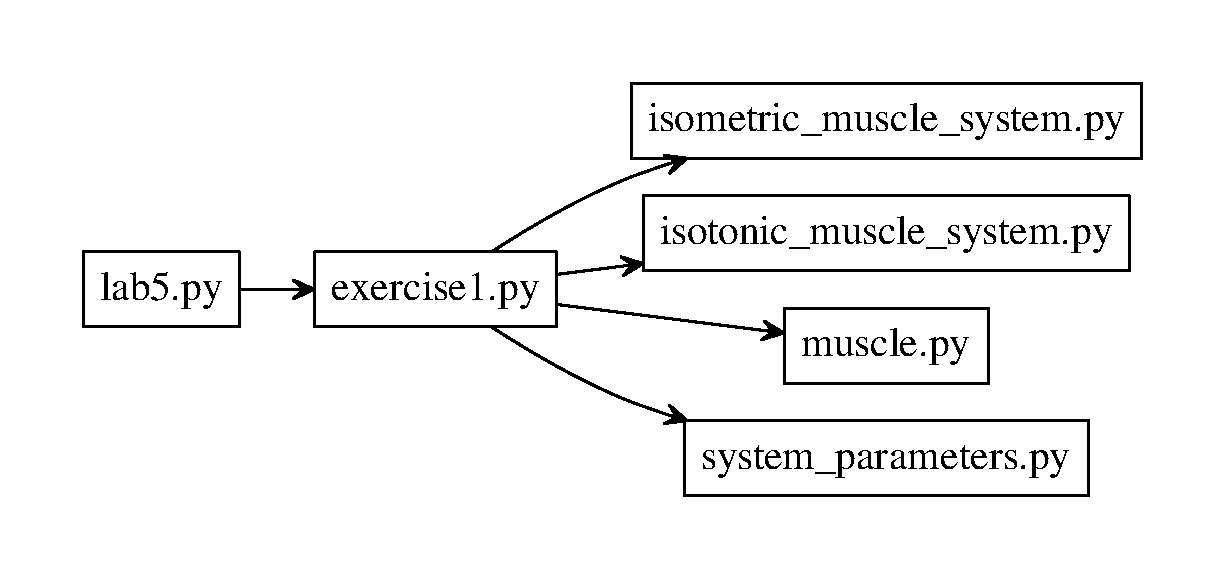
\includegraphics[width=0.5\textwidth]{figures/files_lab5}
  \caption{\label{fig:files_lab5} Exercise files dependencies. In this
  lab, you will be modifying \fileref{exercise1.py}.}
\end{figure}

\subsection*{Files to complete the exercises}
\label{sec:intro_lab5}

\begin{itemize}
\item \fileref{lab5.py} : Main file
\item \fileref{exercise1.py} : Main file to complete exercise 1
\item \fileref{system\_parameters.py} : Parameter class for Pendulum,
  Muscles and Neural Network (Create an instance and change properties
  using the instance. You do not have to modify the file)
\item \fileref{isometric\_muscle\_system.py} : Class to setup your
  isometric muscle test experiments
\item \fileref{isotonic\_muscle\_system.py} : Class to setup your
  isotonic muscle test experiments
\item \fileref{muscle.py} : Muscle class (You do not have to modify
  the file)
\end{itemize}

\textbf{NOTE : } '\textit{You do not have to modify}' does not mean
you should not, it means it is not necessary to complete the
exercises. But, \corr{you are expected to look into each of these
  files and understand how everything works}. You are free to explore
and change any file if you feel so.

\newpage
\section*{Exercise 1 : Hill muscle model}
\label{sec:question-2}

Previous week you explored the role of different passive components
and the effects of its parameters on the system. In this exercise, we
try to understand the contractile or the active element of the hill
muscle model. The components of the hill muscle are described in
figure \ref{fig:hill_muscle}. The equations used to model the hill
muscle can be found in the pdf \fileref{HillMuscleEquations.pdf}

\begin{figure}[H]
  \centering 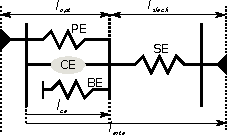
\includegraphics[scale=2.5]{figures/hill_muscle}
  \caption{Hill muscle model}
  \label{fig:hill_muscle}
\end{figure}

Where,

\begin{itemize}
\item $PE$ : Parallel element (Prevents muscle from over stretching)
\item $BE$ : Muscle Belly (Prevents muscle from collapsing on itself)
\item $SE$ : Series element or the muscle tendon element
\item $CE$ : Contractile Element or the active element
\item $l_{opt}$ : Muscle optimal fiber length
\item $l_{slack}$ : Muscle tendon slack length
\item $l_{CE}$ : Contractile element length
\item $l_{MTC}$ : Muscle Tendon Complex length
\end{itemize}


\begin{figure}[H]
  \centering
  \begin{subfigure}[b]{0.49\textwidth}
    { \centering
      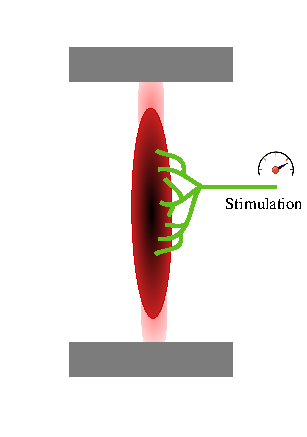
\includegraphics[width=\textwidth]{figures/isometric_muscle} }
    \caption{Isometric muscle setup :\\ To study the relationship
      between Force-Length.}
    \label{fig:isometric_muscle}
  \end{subfigure}
  \begin{subfigure}[b]{0.49\textwidth}
    { \centering
      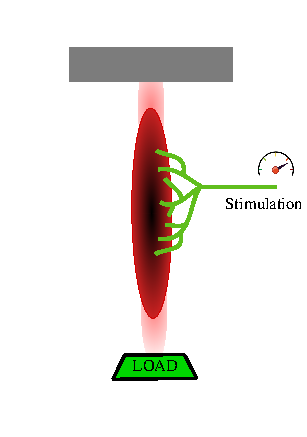
\includegraphics[width=\textwidth]{figures/isotonic_muscle} }
    \caption{Isotonic muscle setup :\\ To study the relationship
      between Force-Velocity.}
    \label{fig:isotonic_muscle}
  \end{subfigure}
  \caption{Muscle Length-Velocity-Force Setup}
  \label{fig:muscle-setup}
\end{figure}

\subsection*{Muscle Force-Length Relationship}
\label{sec:muscle-force-length}
In this exercise you will explore the relation between the length and
velocity of the muscle. In order to do this we replicate the set-up
show in figure \ref{fig:muscle-setup}. Here the length of the muscle is
held constant by attaching it's tendon to two fixed points. While
applying a constant stimulation, observing the force produced will
give the relationship between muscle contractile element length and
force.
\subsection*{1.a For a given stimulation, explore the relationship
  between active and passive muscle forces and the length of the
  contractile element.  Plot the force-length relationship curve.
  Discuss the different regions in the plot. Use the
  \fileref{isometric\_muscle\_system.py::IsometricMuscleSystem} instance
  to setup your experiment in \fileref{exercise1.py}}

To explore the relationship between contractile element length and the active and passive muscle forces, simulated muscles were stretched over a range of lengths between 18 and 30 cm. Muscles were simulated over 0.3 s which was found to be long enough to reach the steady state condition for isometric activation. Stimulation was set to 1.0. All other values were left as the defaults ($l_{slack} = 13 cm, l_{opt} = 11 cm, f_{max} = 1500 N, v_{max} = -12 m/s$, pennation = $1$). Muscles were found to quickly reach steady state length and force. For the isometric case, we were not particularly interested in the transient behaviour, and instead looked at the steady-state force-length relationship. The plot below compares active, passive, and net force generated by the muscle for different lengths of the contractile element.

\begin{figure}[H]
  \centering
    { \centering
      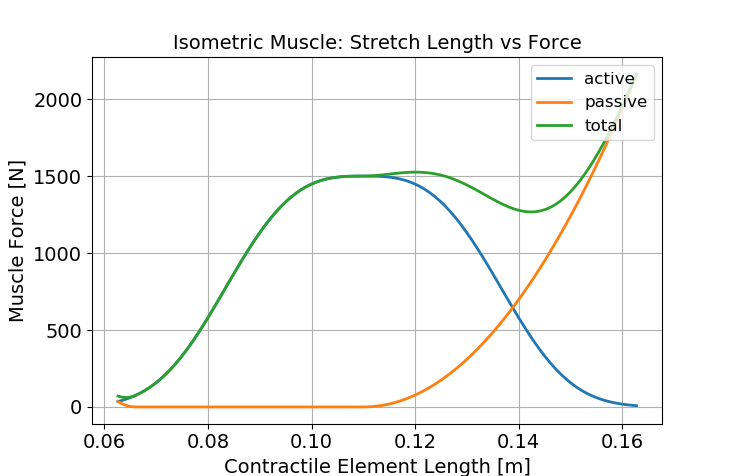
\includegraphics[width=0.75\textwidth]{1a/1a.png}}
    \caption{Steady-state active, passive, and total force generation for different contractile element lengths.}
    \label{fig:f-vs-L}
\end{figure}

In the figure \ref{fig:f-vs-L}, 4 distinct regions exist. The first region at the leftmost point on the graph shows active and passive forces being equal. This indicates a balance between the belly element and the contractile element which prevents the muscle from collapsing. Next, in the region shown between $l_{ce}$ of 0.06 m and 0.11 m, the contractile element is stimulated to produce a force, but the muscle is not stretched enough for the parallel elements or compressed enough for the belly element to be engaged. As such, the passive force is 0 and the active muscle stimulation dominates the force response. The active force generation increases with contractile element length until the max force is reached at 1500 N. This occurs at the optimal length of 11 cm. In the next region, the active muscle force is decreasing, having exceeded the optimal length, while the passive force begins to increase, due to the parallel element engaging. This results in a peak total force at around 12 cm. From 12cm to around 14 cm, the total force drops as the decaying active force still dominates the passive force. However, at 14 cm, the passive force growth rate exceeds the decay of the active force and the total force again increases. In this region, the muscle activation plays a minimal role, and the muscle's elasticity supports nearly all the load. 

\subsection*{1.b In (1.a), you explored the muscle force-length
  relationship for a given stimulation. What happens to the
  relationship when the stimulation is varied between [0 - 1]? Support
  your response with one plot showing the different force-length
  relationship curves.}

In this experiment, rather than changing the length of the muscle, the level of stimulation is changed between 0 and 100\%. This process is repeated for several muscle lengths to investigate the effect for different muscle responses. Again, default muscle parameters are used. The active, passive, and net forces are plotted for 4 different MTU lengths: 12cm, 18cm, 24cm, and 30cm. Surface plots of the active and passive force generation for different stimulations and muscle lengths are included in Figures \ref{fig:stimForcea} and \ref{fig:stimForceb}.

\begin{figure}[H]
    \begin{subfigure}{.48\textwidth}
        \centering
          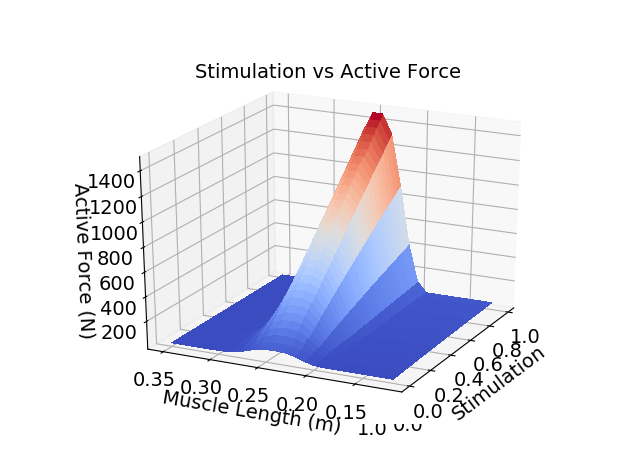
\includegraphics[width=\textwidth]{1b/1b._Stim_vs_Active_Force_Surface_Plot.png}
        \subcaption{Effect of Stimulation (right) and Muscle Stretch (left) on Active Muscle Force (vertical).}
    \label{fig:stimForcea}
    \end{subfigure}    
    \hfill
    \begin{subfigure}{.48\textwidth}
        \centering
          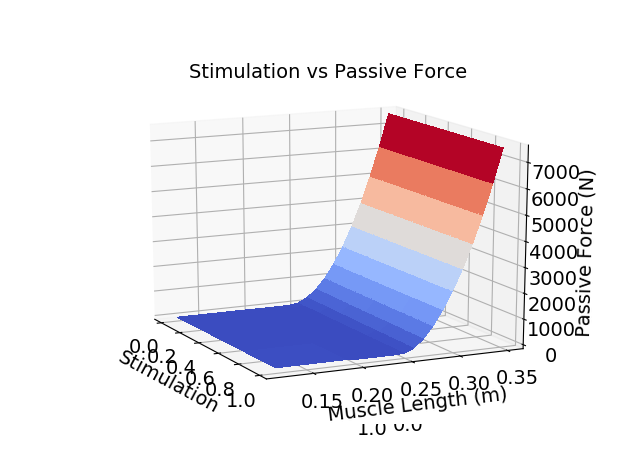
\includegraphics[width=\textwidth]{1b/1b._Stim_vs_Passive_Force_Surface_Plot.png}
        \subcaption{Effect of Stimulation (Left) and Muscle Stretch (Right) on Passive Muscle Force (vertical).}
    \label{fig:stimForceb}
    \end{subfigure}
\end{figure}

As can be seen in  Figures \ref{fig:stimForcea} and \ref{fig:stimForceb}, stimulation has no impact on passive force generation of the muscle, as could be expected. However the effect of stimulation on active force is interesting to discuss. Muscle force increases linearly with stimulation for all muscle stretch values. However, when the contractile element is near it's optimal length, the active force generation increases. Referencing the Hill Muscle Equations used in the model, it is indeed an exponential decay of the muscle stretch cubed. As such, the force is near max around the optimal muscle length, and quickly decays to nearly zero away from that length, indicating that the muscles have a very narrow active range. 

\subsection*{1.c Describe how the fiber length ($l_{opt}$) influences
  the force-length curve. (Compare a muscle comprised of short muscle
  fibers to a muscle comprised on long muscle fibers.). To change the
  parameter you can use
  \fileref{system\_parameters.py::MuscleParameters} before
  instantiating the muscle. No more than two plots are required. }

In this section, the influence of optimal length on the force-length curve was investigated. Stimulation was kept constant at 1. For each optimal length, a force-stretch curve was plotted for both active and passive forces. Figure \ref{fig:loptForce} shows the isometric muscle forces for different optimal muscle lengths. 

\begin{figure}[H]
    \centering
    \begin{subfigure}{.48\textwidth}
        \centering
          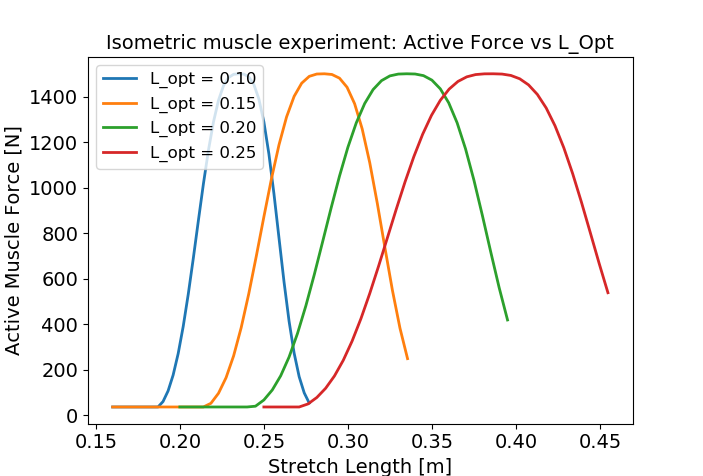
\includegraphics[width=\textwidth,trim={0.0cm 0.0cm 1.0cm 0.0cm},clip]{1c/1c_active.png}
    \end{subfigure}    
    \begin{subfigure}{.48\textwidth}
        \centering
          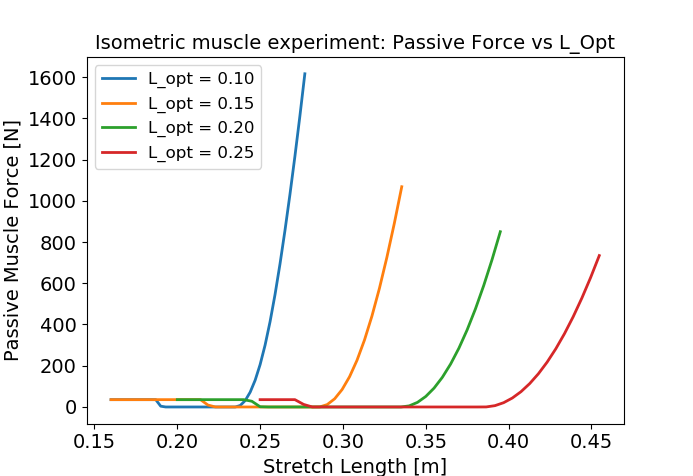
\includegraphics[width=0.98\textwidth,trim={0.0cm 0.0cm 1.0cm 0.0cm},clip]{1c/1c_passive.png}
    \end{subfigure}
    \caption{Effect of Optimal Length on Active (left) and Passive (right) Muscle Force for Different Stretch Lengths.}
    \label{fig:loptForce}
\end{figure}

As the active muscle force is limited to 1500 N, the peak active force for the muscles of different length do not change. However, what is interesting is that the longer muscles are able to generate large forces for a broader range of muscle stretch value. The larger muscles also have more gradual growth and decay rates.\\ 

Looking at the passive force plot to the right, there are again some interesting differences to note. For instance, all the muscles react with the same force to being over-compressed. Each muscles has a region of zero-passive-force. This region's size is related to the muscle length, with the 0.25m $l_{opt}$ muscle having a zero passive force region which is about 0.11m long compared to the shortest 0.10m $l_{opt}$ muscle where the region was only about 0.05m long. This region appears to scale linearly. Again, the growth rate of the force is related to the optimal length, with shorter muscles growing at higher rates. This is due to the fact that the force is related to the change in length of the muscle proportional to the optimal length of the muscle. Longer muscles require more stretch to achieve the same proportion.

\subsection*{Muscle Velocity-Tension Relationship}
In this exercise you will explore the relation between the force and
velocity of the muscle. In order to do this we replicate the set-up
show in figure \ref{fig:muscle-setup}. Here the length of the muscle
is allowed to vary by attaching one of its end to a fixed point and
the other to a variable external load. While applying a constant load
initially and holding the muscle at constant length, a quick release
is performed to let the muscle contract and pull the weight. The
maximum velocity during this quick release will give us the
relationship between muscle contractile velocity and the force.


\corr{Note} : Since the velocity changes sign and you need to compute the maximum
velocity accordingly by checking if the muscle was stretched or compressed
at the end of the experiment.

\begin{equation}
  \label{eq:2_lab5}
 V_{ce} = \left\{
\begin{array}{ll}
      max(v_{ce}(t)) & l_{mtc} < (l_{opt} + l_{slack}) \\
      min(v_{ce}(t)) & else \\
\end{array}
\right.
\end{equation}

\subsection*{1.d For a stimulation of 1.0 and starting at optimal
  muscle length, explore the relationship between contractile element
  velocity and external load. Plot the Velocity - Tension relationship
  curve. Include shortening and lengthening regions. Use the
  \fileref{isotonic\_muscle\_system.py::IsotonicMuscleSystem} instance
  to setup your experiment in \fileref{exercise1.py}}
  
As shown in figures \ref{fig:isotonic_load} \textit{a} and \textit{b} there is three types of situation:
\begin{enumerate}
    \item Between 5 and around 100 newtons the load is much lower than the muscle force applied so as soon as the muscle is released it will contract quickly (then bumped).
    \item Between around 100 and 200 newtons the load is quiet the same as the muscle force applied so the velocity of the muscle is low. It is also zero at the load value $152.2$ [N].
    \item At more than 200 newtons the load is much higher than the muscle force applied so it will have high positive velocity. It still come back to a stable state as demonstrate with a velocity null after $1.1$ second maximum.
    
\end{enumerate}
\begin{figure}[H]
    \centering
    \begin{subfigure}[b]{0.49\textwidth}
        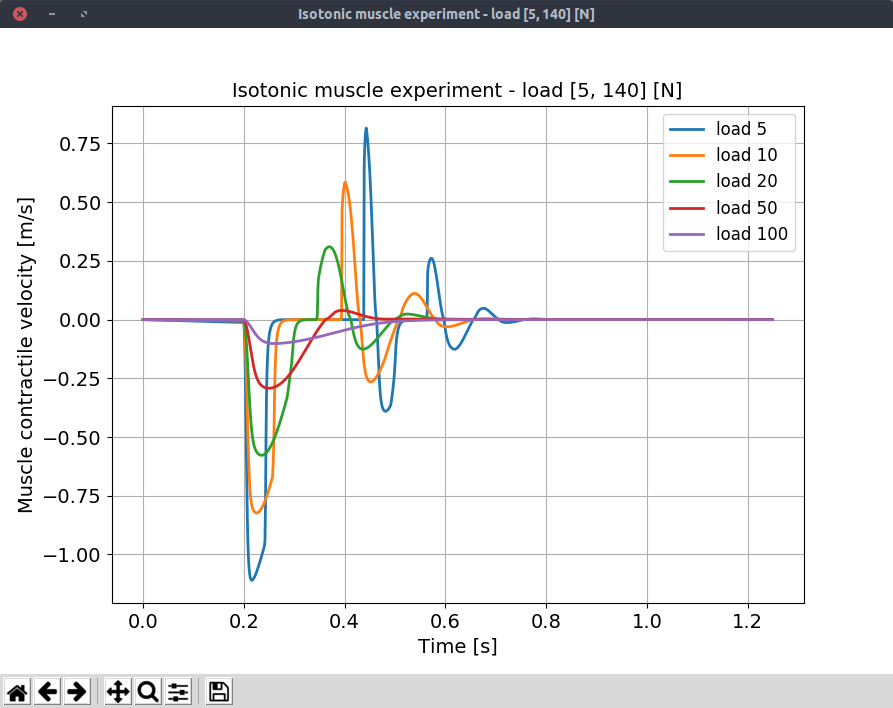
\includegraphics[width=\textwidth,trim={0.5cm 1.25cm 1.5cm 1.5cm},clip]{1d/isotonic_small_load.png}
        \subcaption{Load from 5 to 100 [N]}
    \end{subfigure}
    \begin{subfigure}[b]{0.49\textwidth}
        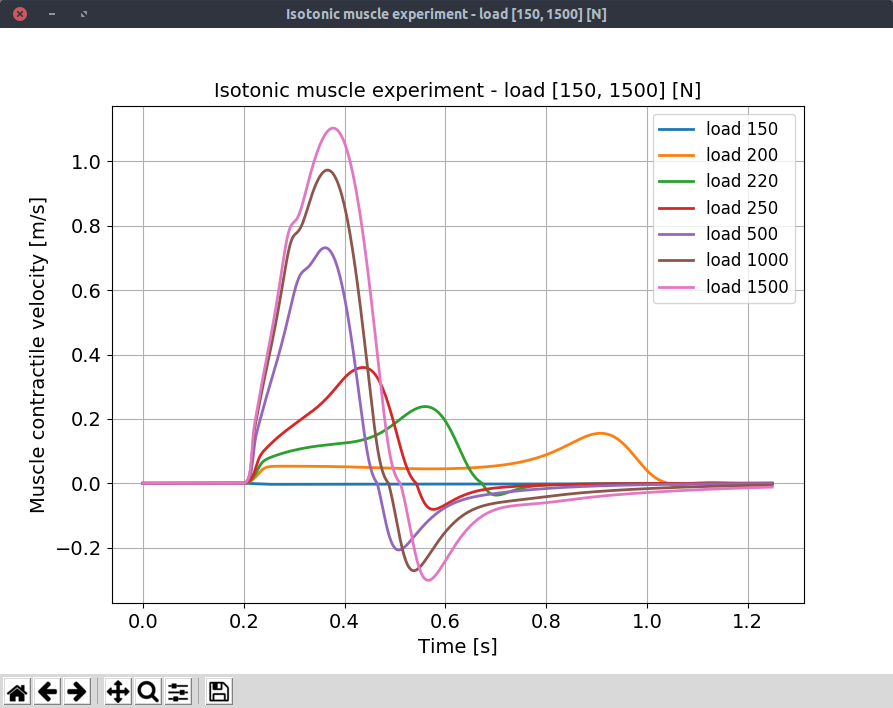
\includegraphics[width=\textwidth,trim={0.5cm 1.25cm 1.5cm 1.5cm},clip]{1d/isotonic_big_load.png}
        \subcaption{Load from 150 to 1500 [N]}
    \end{subfigure}
    \begin{subfigure}[b]{0.55\textwidth}
        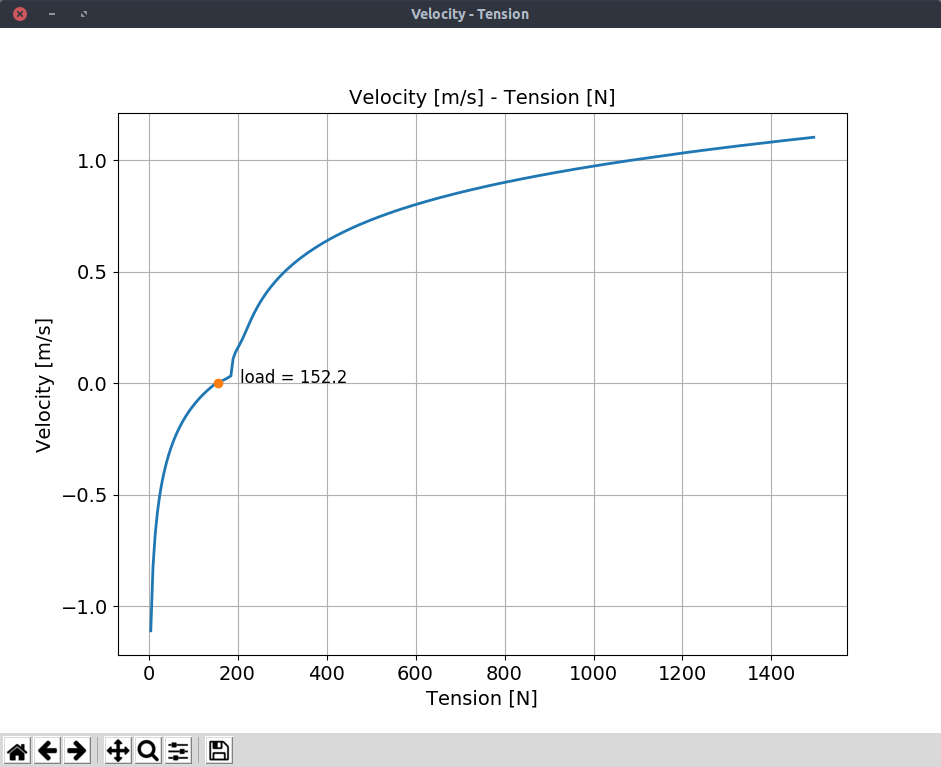
\includegraphics[width=\textwidth,trim={0.5cm 1.25cm 1.5cm 1.5cm},clip]{1d/isotonic_vce_load.png}
        \subcaption{Load from 5 to 1500 [N]}
    \end{subfigure}
    \caption{\textit{UP :} Muscle contractile velocity [m/s] - Time [s] - \textit{DOWN :} Muscle contractile velocity [m/s] - Load [N]}
    \label{fig:isotonic_load}
\end{figure}

To conclude, as shown in figure \ref{fig:isotonic_load} $c$, the maximum velocity over the load applied increase exponentially in negative part for small load mass. Since the load is not big enough, the muscle will directly contract itself as soon as it is released and this is why the value is negative. The velocity will reach to zero at the value where the load exactly compensate the stimulation muscle then continue to increase to tend to its maximum value which is dependent to the $f_{max}$ parameter set. Since the graph is over the load, it will continue to increase after reaching the maximum load value of $1500$ [N] because the simulation does not take into account the ductility of the muscle.

\subsection*{1.e For the muscle force-velocity relationship, why is the lengthening force greater than the force output during shortening? No plots necessary}

The lengthening force is greater than the shortening force as was demonstrated through several experimental results, including Hill's original paper outlining the Hill Muscle Model. The reason for this difference in force is perhaps best discussed by Huxley and Hanson (1953) in their paper on sliding filament theory and the subsequent addition of Cross-Bridge theory, and has to do with the different actions of muscle fibers in concentric (shortening) and eccentric (lengthening) contractions. This is perhaps out of the scope of this course. Mathematically, the explanation is perhaps a bit simpler.

Referencing the Hill Muscle Equations, the equation for the force-velocity relationship, $f_v(v_{ce})$, it can be shown that the equation for the shortening case has a smaller derivative respect to $v_{ce}$. 

Rewriting the shortening force equation (for $v_{ce}<0$) to instead use $-|v_{ce}|$ for $v_{ce}>0$, both parts of the piece-wise can be directly compared. This substitution results in: 
\begin{equation} 
    f_v|_{lengthening}= \frac{v_{max}-v_{ce}}{v_{max}+Kv_{ce}}
\end{equation}
\begin{equation} 
    f_v|_{shortening}= N+(1-N)\frac{v_{max}-v_{ce}}{v_{max}+7.56Kv_{ce}}
\end{equation}

For N=1.5, K>0 and $v_{max}$>0, as used as the default value in the simulations, it is evident that the shortening equation will always have a larger denominator ($2v_{max}+7.56Kv_{ce}>v_{max}+Kv_{ce}$ for all $v_{ce}$) and therefore a smaller force. 

\subsection*{1.f What happens to the force-velocity relationship when the stimulation is varied between [0 - 1]? Support your response with one plot showing the different force-velocity relationship curves.}
  
\begin{figure}[H]
    \centering
    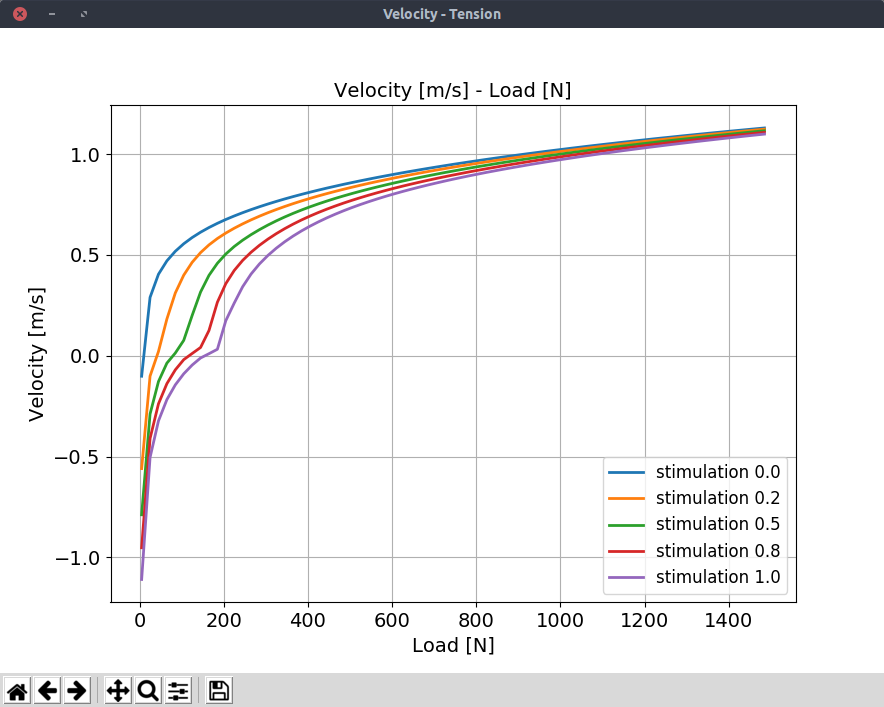
\includegraphics[width=0.75\textwidth,trim={0.5cm 1.25cm 1.5cm 1.5cm},clip]{1f/force_vce_stimulation.png}
    \caption{Force [N] - Velocity [m/s] graph for isotonic muscle with respect to stimulation changes.}
    \label{fig:isotonic_force_velocity}
\end{figure}

As shown in the figure \ref{fig:isotonic_force_velocity}, the muscle will better react if the stimulation is bigger. The fact is that the muscle will not be able to compensate any load if there is no stimulation, as shown with the curve at stimulation zero were the negative part of the velocity is nearly nonexistent. It is also shown that when the muscle is well stimulate, the reaction is responsive and the negative velocity is as high as the maximum positive one.
  
\end{document}

%%% Local Variables:
%%% mode: latex
%%% TeX-master: t
%%% End: